\input templates/header

\graphicspath{{figs/A1/}}

\begin{document}

\title[ASD - Algoritmi di ordinamento]{\textbf{Algoritmi e strutture dati}\\[24pt]Algoritmi di ordinamento}

%-------------------------------------------------------------------------
\FrameTitle{}

%%%%%%%%%%%%%%%%%%%%%%%%%%%%%%%%%%%%%%%%%%%%%%%%%%%%%%%%%%%%%%%%%%%%%%%%%%

\begin{frame}{Introduzione}

\begin{block}{Sommario - Algoritmi di ordinamento}
\begin{columns}
\begin{column}{0.48\textwidth}
\BI
\item SelectionSort - $\Theta(n^2)$
\item InsertionSort - $\Omega(n)$, $O(n^2)$
\item ShellSort - $\Omega(n)$, $O(n^{3/2})$
\EI
\end{column}
\begin{column}{0.48\textwidth} 
\BI
\item MergeSort - $\Theta(n \log n)$
\item HeapSort - $\Theta(n \log n)$
\item QuickSort - $\Omega(n \log n)$, $O(n^2)$
\EI
\end{column}
\end{columns}
\end{block}


\bigskip
\begin{block}{Sommario - Problema dell'ordinamento}
\BI
\item \alert{Tutti questi algoritmi sono basati su confronti}
\BI
\item Le decisioni sull'ordinamento vengono prese in base al confronto ($<$,$=$,$>$) fra due valori
\EI
\item \alert{Algoritmi migliori: $O(n \log n)$}
\BI
\item InsertionSort e ShellSort sono più veloci solo in casi speciali
\EI
\EI
\end{block}

\end{frame}


\begin{frame}{Introduzione}

\begin{block}{Problema dell'ordinamento - Limite inferiore}
E' possibile dimostrare che qualunque algoritmo di ordinamento \alert{basato su confronti} ha una complessità 
$\Omega(n \log n)$.
\end{block}

\begin{block}{Assunzioni}
\BI
\item Consideriamo un qualunque algoritmo $A$ basato su confronti
\item Assumiamo che tutti i valori siano distinti (no perdita di generalità)
\item L'algoritmo $A$  può essere rappresentato tramite un \alert{albero di decisione}, un albero binario che rappresenta i confronti fra gli elementi
\EI
\end{block}

\end{frame}%%%%%%%%%%%%%%%%%%%%%%%%%%%%%%%%%%%%%%%%%%%%%%%%%%%%%%%%%%%%%%%%%%%%%%%%%%%%%%%%%%%%%%%%%%%%

\begin{frame}{Albero di decisione}
	
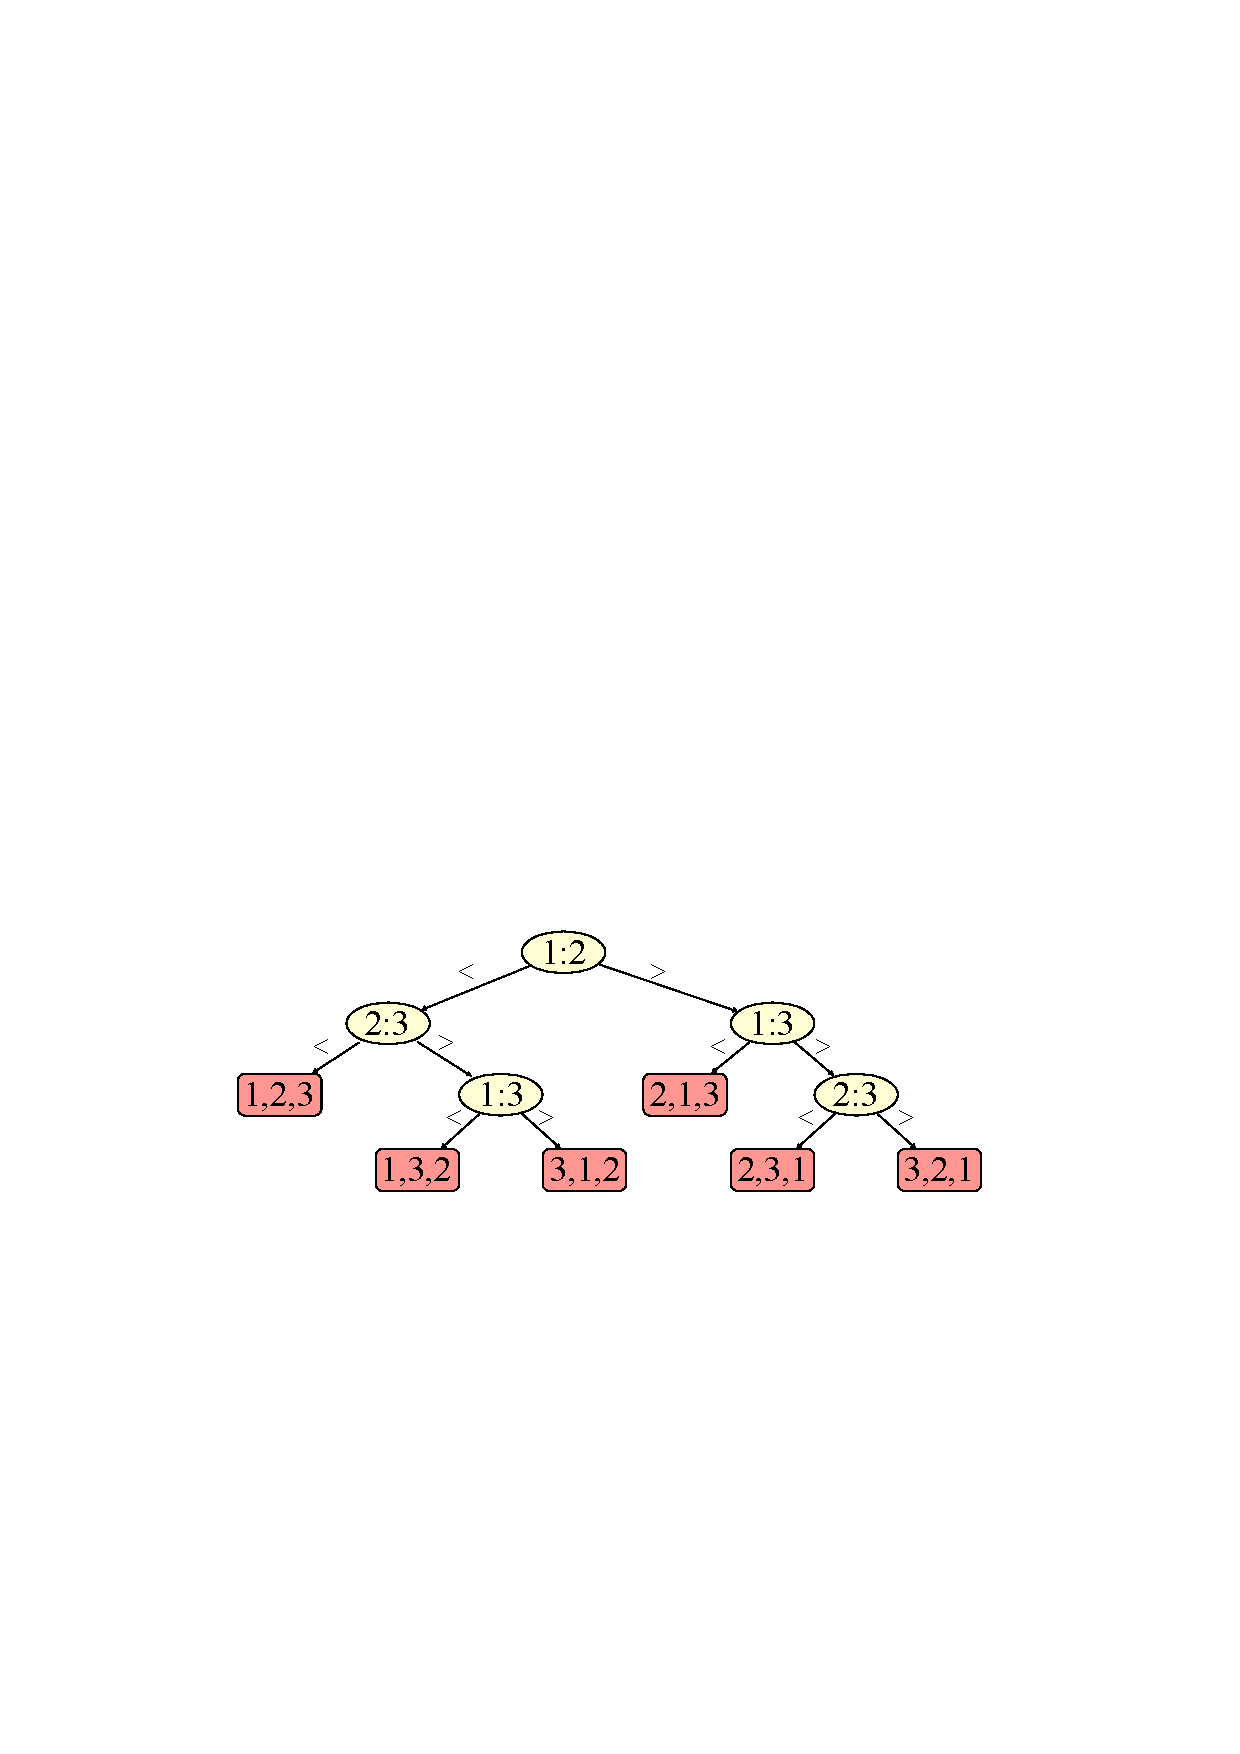
\includegraphics[width=\textwidth]{albero-ordinamento.pdf}	
	
\end{frame}%%%%%%%%%%%%%%%%%%%%%%%%%%%%%%%%%%%%%%%%%%%%%%%%%%%%%%%%%%%%%%%%%%%%%%%%%%%%%%%%%%%%%%%%%%%%

\begin{frame}{Albero di decisione}
	
\begin{block}{Proprietà}
\BI
\item \alert{Cammino radice-foglia in un albero di decisione}: sequenza di confronti eseguiti dall'algoritmo corrispondente
\item \alert{Altezza dell'albero di decisione}: numero confronti eseguiti dall'algoritmo corrispondente nel caso pessimo
\EI
\end{block}

\bigskip
Si considerino tutti gli alberi di decisioni ottenibili da algoritmi di ordinamento basati su confronti

\end{frame}%%%%%%%%%%%%%%%%%%%%%%%%%%%%%%%%%%%%%%%%%%%%%%%%%%%%%%%%%%%%%%%%%%%%%%%%%%%%%%%%%%%%%%%%%%%%

\begin{frame}{Limite inferiore per l'ordinamenento}

\begin{block}{Lemma 1}
Un albero di decisione per l'ordinamento di $n$ elementi contiene almeno $n!$ foglie
\end{block}

\begin{block}{Lemma 2}
Sia $T$ un albero binario in cui ogni nodo interno ha esattamente $2$ figli e sia $k$ il numero delle sue foglie. 
L'altezza dell'albero è almeno $\log k$ - ovvero $\Omega(\log k)$.
\end{block}

\begin{block}{Teorema}
Il numero di confronti necessari per ordinare n elementi nel caso peggiore è $\Omega(n \log n)$
\end{block}

\end{frame}%%%%%%%%%%%%%%%%%%%%%%%%%%%%%%%%%%%%%%%%%%%%%%%%%%%%%%%%%%%%%%%%%%%%%%%%%%%%%%%%%%%%%%%%%%%%


\begin{frame}{Spaghetti Sort}

\begin{block}{Algoritmo Spaghetti Sort -- $O(n)$}
\begin{enumerate}
\item Prendi $n$ spaghetti
\item Taglia lo spaghetto $i$-esimo in modo proporzionale all'$i$-esimo valore da ordinare
\item Con la mano, afferra gli $n$ spaghetti e appoggiali verticalmente sul tavolo
\item Prendi il più lungo, misuralo e metti il valore corrispondente in fondo al vettore da ordinare
\item Ripeti (4) fino a quando non hai terminato gli spaghetti
\end{enumerate}
\end{block}
\end{frame}%%%%%%%%%%%%%%%%%%%%%%%%%%%%%%%%%%%%%%%%%%%%%%%%%%%%%%%%%%%%%%%%%%%%%%%%%%%%%%%%%%%%%%%%%%%%

\begin{frame}{Counting Sort}
Assunzione:
\BI
\item I numeri da ordinare sono compresi in un intervallo $[1 \ldots k]$
\EI

\bigskip
Come funziona:
\BI
\item  Costruisce un array $B[1 \ldots k]$ che conta il numero di volte che un valore compreso in $[1 \ldots k]$ compare in $A$
\item Ricolloca i valori così ottenuti nel vettore da ordinare  $A$	
\EI

\bigskip
Miglioramenti:
\BI
\item L'intervallo non deve necessariamente iniziare in $1$ e finire in $k$; qualunque intervallo di cui conosciamo gli estremi può essere utilizzato
nel Counting Sort.
\EI
\end{frame}%%%%%%%%%%%%%%%%%%%%%%%%%%%%%%%%%%%%%%%%%%%%%%%%%%%%%%%%%%%%%%%%%%%%%%%%%%%%%%%%%%%%%%%%%%%%


\begin{frame}{Counting Sort}

\begin{Procedure}
\caption[A]{\countingsort($\INTEGER[\,]\ A,\ \INTEGER\ n,\ \INTEGER\ k$)}
$\INTEGER[\,]\ B = \NEW\ \INTEGER[1 \mldots k]$\;
\For{$i = 1$ \TO\ $k$}{$B[i] = 0$\;}
\For{$j = 1$ \TO\ $n$}
{
  $B[A[j]] = B[A[j]]+1$\;
}
$j = 1$\;
\For{$i = 1$ \TO\ $k$}
{
  \While{$B[i]>0$}
  {
    $A[j] = i$\;
    $j = j+1$\;
    $B[i] = B[i]-1$\;
  }
}
\end{Procedure}


\end{frame}%%%%%%%%%%%%%%%%%%%%%%%%%%%%%%%%%%%%%%%%%%%%%%%%%%%%%%%%%%%%%%%%%%%%%%%%%%%%%%%%%%%%%%%%%%%%

\begin{frame}{Counting Sort}
	
\begin{block}{Complessità di Counting Sort}
\BI
\item $O(n+k)$
\item Se $k$ è $O(n)$, allora la complessità di Counting Sort è $O(n)$
\EI
\end{block}

\bigskip
\begin{block}{Counting Sort e limiti inferiore per l'ordinamento}
\BI
\item Counting Sort non è basato su confronti
\item Abbiamo cambiato le condizioni di base 
\item Se $k$ è $O(n^3)$, questo algoritmo è peggiore di tutti quelli visti finora	
\EI
\end{block}
\end{frame}%%%%%%%%%%%%%%%%%%%%%%%%%%%%%%%%%%%%%%%%%%%%%%%%%%%%%%%%%%%%%%%%%%%%%%%%%%%%%%%%%%%%%%%%%%%%

\begin{frame}{Pigeonhole Sort}

\begin{block}{Casellario}
\BI
\item Cosa succede se i valori non sono numeri interi, ma record associati ad una chiave da ordinare?
\item Non possiamo usare counting
\item Ma possiamo usare liste concatenate!
\EI
\end{block}

\bigskip
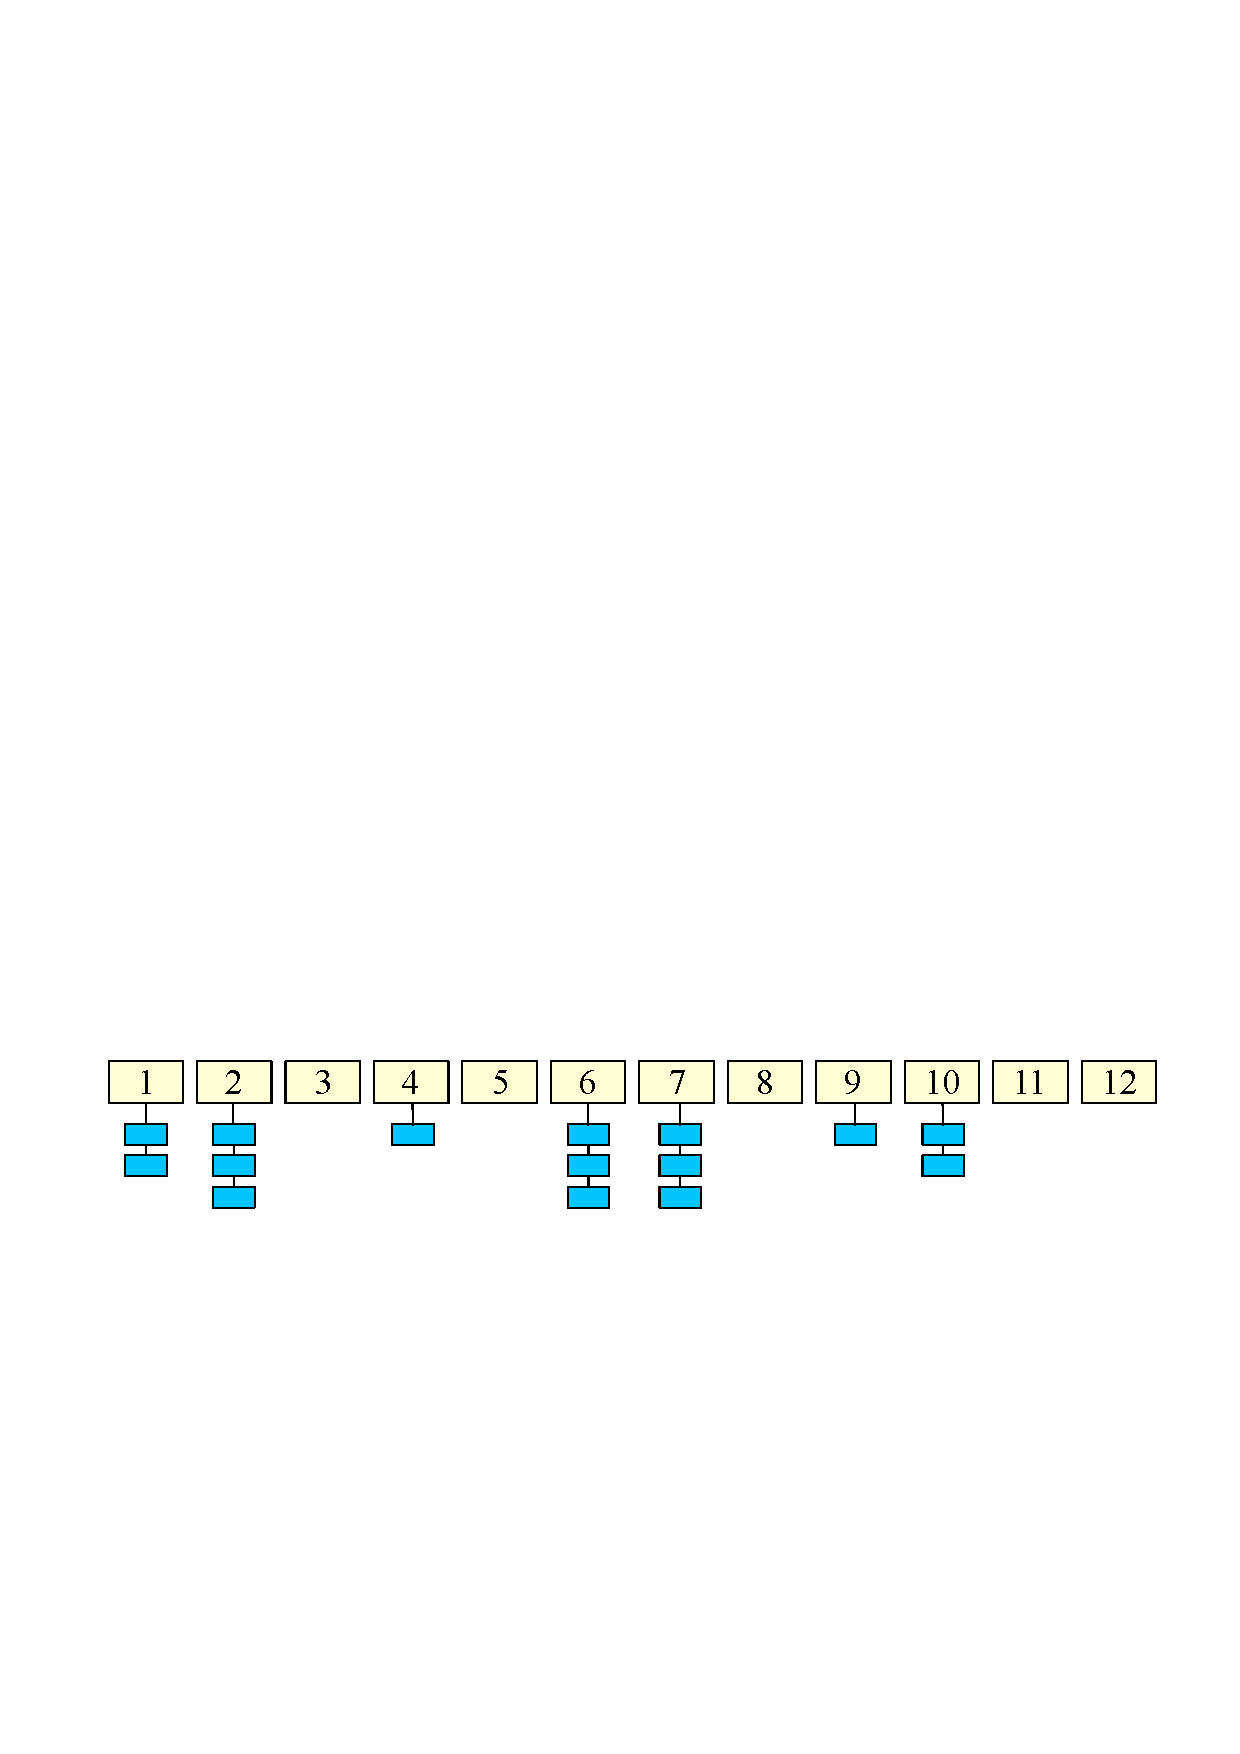
\includegraphics[width=\textwidth]{pigeonhole.pdf}	

\end{frame}%%%%%%%%%%%%%%%%%%%%%%%%%%%%%%%%%%%%%%%%%%%%%%%%%%%%%%%%%%%%%%%%%%%%%%%%%%%%%%%%%%%%%%%%%%%%

\begin{frame}[shrink]{Bucket Sort}

\begin{block}{Ipotesi sull'input}
\BI
\item Valori reali uniformemente distribuiti nell'intervallo $[0, 1)$
\item Qualunque insieme di valori distribuiti uniformemente può essere normalizzato nell'intervallo $[0, 1)$ in tempo lineare
\EI
\end{block}

\begin{block}{Idea}
\BI
\item Dividere l'intervallo in $n$ sottointervalli di dimensione $1/n$, detti \alert{bucket}, e poi distribuire gli $n$ numeri nei bucket
\item Per l'ipotesi di uniformità, il numero atteso di valori nei bucket è $1$
\item Possono essere ordinati con Insertion Sort
\EI
\end{block}

\bigskip
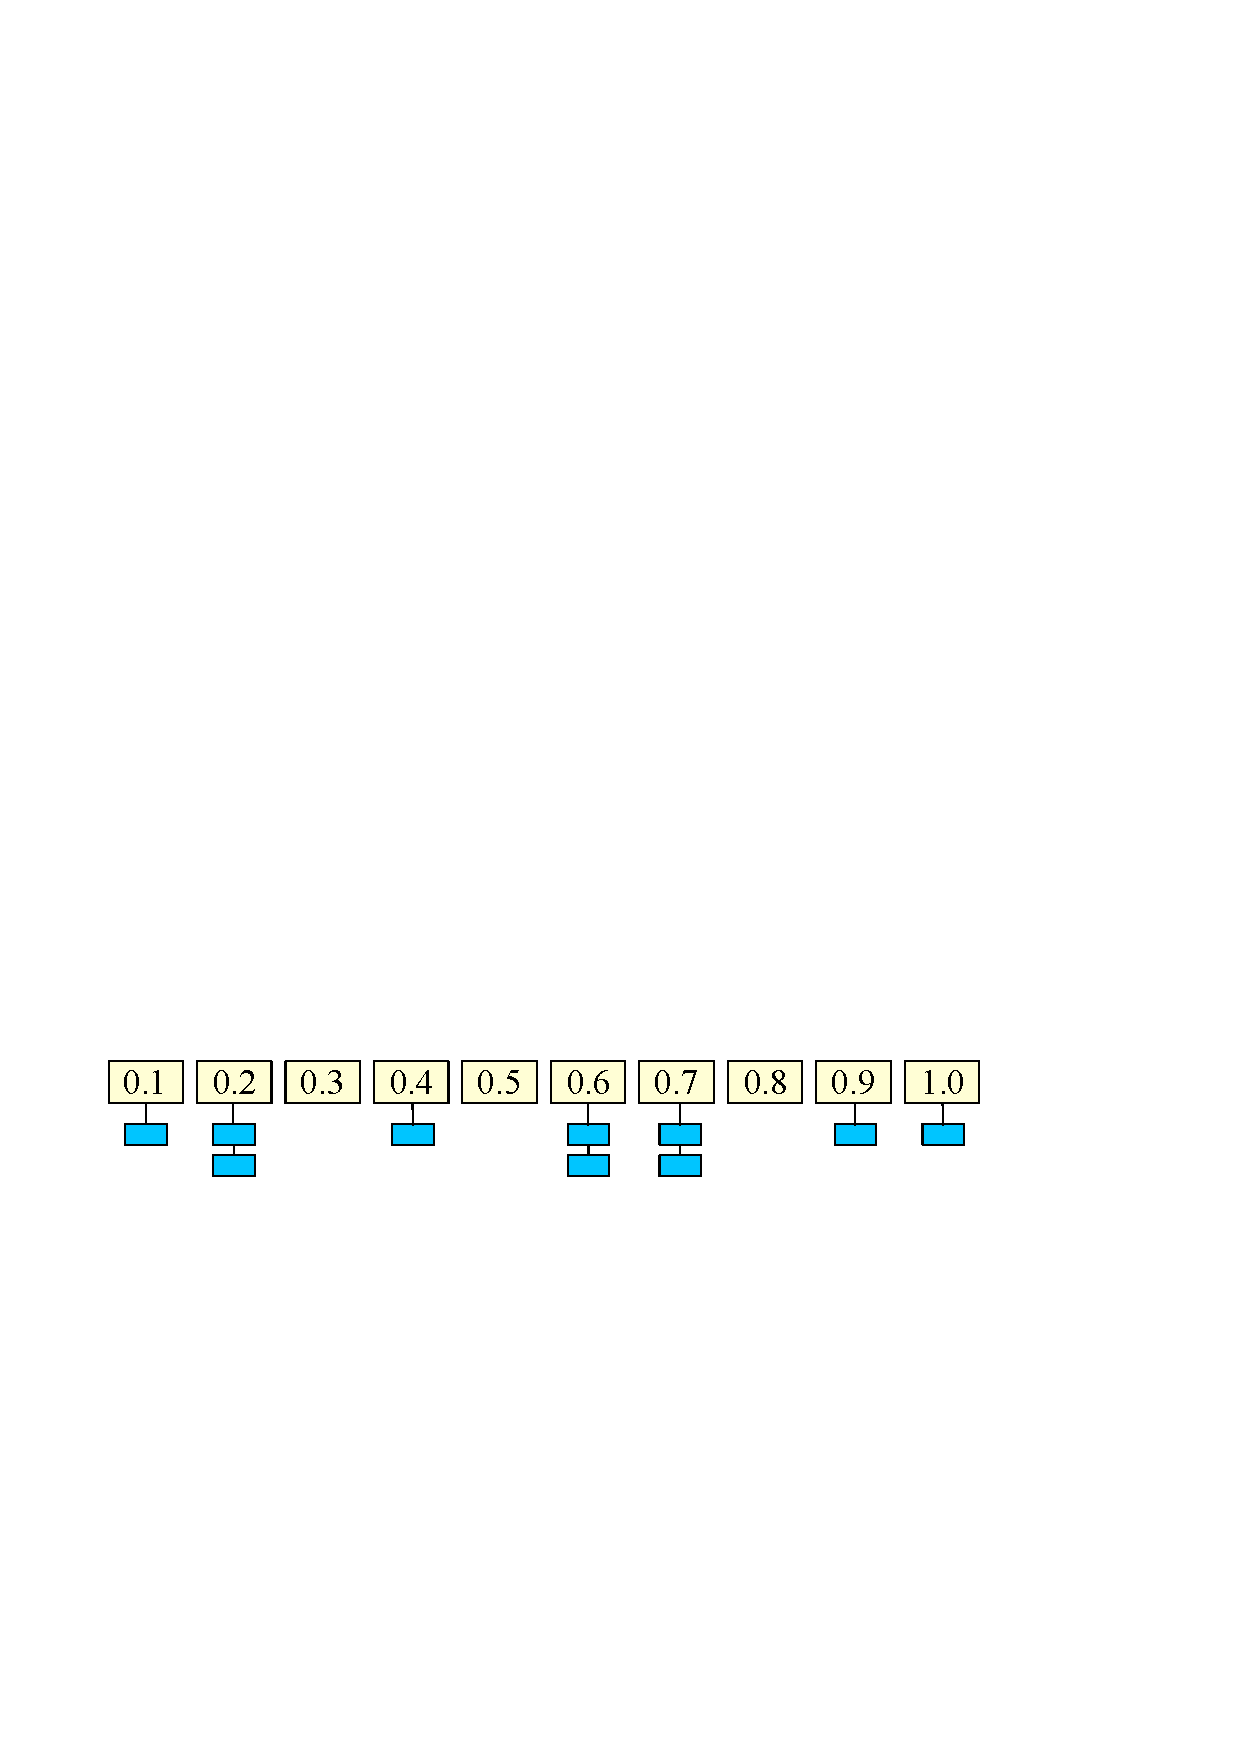
\includegraphics[width=\textwidth]{bucket.pdf}	

\end{frame}%%%%%%%%%%%%%%%%%%%%%%%%%%%%%%%%%%%%%%%%%%%%%%%%%%%%%%%%%%%%%%%%%%%%%%%%%%%%%%%%%%%%%%%%%%%%


\begin{frame}{Proprietà degli algoritmi di ordinamento}
\begin{block}{Stabilità}
Un algoritmo di ordinamento è \alert{stabile} se preserva l'ordine iniziale tra due elementi con la stessa chiave
\end{block}

\bigskip
\begin{block}{Domande}
\BI
\item Quali dei seguenti algoritmi sono stabili? Insertion Sort, Merge Sort, Heap Sort, Quick Sort, Pigeonhole Sort
\item Come si può rendere un qualunque algoritmo stabile?
\EI
\end{block}

\pause
\bigskip
\begin{block}{Risposte}
\BI
\item Stabili: Insertion Sort, Merge Sort, Pigeonhole Sort
\item  Basta usare come chiave di ordinamento la coppia\\ (chiave, posizione iniziale) 
\EI
\end{block}
\end{frame}%%%%%%%%%%%%%%%%%%%%%%%%%%%%%%%%%%%%%%%%%%%%%%%%%%%%%%%%%%%%%%%%%%%%%%%%%%%%%%%%%%%%%%%%%%%%

\begin{frame}{Riassunto ordinamento}
\begin{block}{Insertion Sort}
$\Omega(n)$, $O(n^2)$, stabile, sul posto, iterativo. Adatto per piccoli valori, sequenze quasi ordinate.
\end{block}
\begin{block}{Merge Sort} 
$\Theta(n\log n)$, stabile, richiede $O(n)$ spazio aggiuntivo, ricorsivo (richiede $O(\log n)$ spazio nello stack). Buona performance in cache, buona parallelizzazione.
\end{block}
\begin{block}{Heap Sort}
$\Theta(n\log n)$, non stabile, sul posto, iterativo. Cattiva performance in cache, cattiva parallelizzazione. Preferito in sistemi embedded.
\end{block}
\end{frame}%%%%%%%%%%%%%%%%%%%%%%%%%%%%%%%%%%%%%%%%%%%%%%%%%%%%%%%%%%%%%%%%%%%%%%%%%%%%%%%%%%%%%%%%%%%%

\begin{frame}{Riassunto ordinamento}
\begin{block}{Quick Sort}
$O(n\log n)$ in media, $O(n^2)$ nel caso peggiore, non stabile, ricorsivo (richiede $O(\log n)$ spazio nello stack). Buona performance in cache, buona parallelizzazione, buoni fattori moltiplicativi.
\end{block}
\begin{block}{Counting Sort}
$\Theta(n+k)$, richiede $O(k)$ memoria aggiuntiva, iterativo. Molto veloce quando $k=O(n)$
\end{block}
\begin{block}{Pigeonhole Sort}
$\Theta(n+k)$, stabile, richiede $O(n+k)$ memoria aggiuntiva, iterativo. Molto veloce quando $k=O(n)$
\end{block}
\end{frame}%%%%%%%%%%%%%%%%%%%%%%%%%%%%%%%%%%%%%%%%%%%%%%%%%%%%%%%%%%%%%%%%%%%%%%%%%%%%%%%%%%%%%%%%%%%%

\begin{frame}{Riassunto ordinamento}
\begin{block}{Bucket Sort}
$O(n)$ nel caso i valori siano distribuiti uniformemente, stabile, richiede $O(n)$ spazio aggiuntivo
\end{block}

\begin{block}{Shell Sort}
$O(n \sqrt{n})$, stabile, adatto per piccoli valori, sequenze quasi ordinate.
\end{block}

\end{frame}%%%%%%%%%%%%%%%%%%%%%%%%%%%%%%%%%%%%%%%%%%%%%%%%%%%%%%%%%%%%%%%%%%%%%%%%%%%%%%%%%%%%%%%%%%%%

\begin{frame}{Reality check}
\begin{block}{Tim Sort}
\BI
\item Algoritmo ibrido, basato su Merge Sort e Insertion Sort
\item Cerca sequenze consecutive (run) già ordinate 
\item Complessità: 
\BI
\item $\Omega(n)$ (sequenze già ordinate)
\item $O(n \log n)$ nel caso pessimo
\EI
\EI
\end{block}

\begin{block}{Utilizzazione}
\BI
\item Python
\item Java 7
\item Gnu Octave
\EI
\end{block}

\end{frame}%%%%%%%%%%%%%%%%%%%%%%%%%%%%%%%%%%%%%%%%%%%%%%%%%%%%%%%%%%%%%%%%%%%%%%%%%%%%%%%%%%%%%%%%%%%%



\end{document}